\section{Introduction}
\label{sec:intro}

% 第一段 ： Text-to-SQL 的背景
Text-to-SQL aims to translate natural language (NL) questions into executable SQL queries, enabling non-expert users to retrieve and analyze relational data without manually writing database programs~\cite{androutsopoulos1995natural,hendrix1978developing,popescu2003towards}. 
Its importance has grown with increasingly large schemas, rich database contents, and diverse analytical tasks, motivating benchmarks such as \textsc{Spider}~\cite{yu2018spider}, \textsc{BIRD}~\cite{li2023can}. 
Recent LLM-based systems have achieved substantial progress through in-context learning, task decomposition and specialized agents, moving the field beyond single-shot generation toward workflow-based SQL construction~\cite{gao2023text,pourreza2023din,wang2023mac,talaei2024chess}.


% 第二段：现有 Text-to-SQL 典型工作流
\textbf{From Single-shot Generation to Agentic Workflows.}
As shown in Figure~\ref{fig:text-to-sql-pipeline}, modern Text-to-SQL systems typically organize SQL construction into three stages: pre-generation, generation, and post-generation.
In the pre-generation stage, the system grounds the natural language query in the database context through schema linking, value grounding, and information retrieval, thereby reducing the search space and enriching the input evidence~\cite{talaei2024chess,lewis2020retrieval,pham2026avsql,biswal2026agentsm}. 
In the generation stage, the model applies prompting strategies, query planning, and LLM-based reasoning to produce one or more candidate SQL queries~\cite{gao2023text,pourreza2023din,wang2023mac,chaturvedi2025sqlthought,heidari2025agentiql,yang2025marssql}. 
In the post-generation stage, these candidates are further checked and refined through execution validation, repair, and consistency- or ensemble-based selection~\cite{wang2022selfconsistency,pourreza2023din,yao2023react,wang2023mac,talaei2024chess,chaturvedi2025sqlthought,heidari2025agentiql,yang2025marssql}.
Compared with single-pass generation, such workflows are more robust because they decompose SQL construction into modular steps, strengthen database grounding, diversify candidate generation, and provide post-hoc opportunities for validation and refinement. 
%
%\textbf{Limitations of existing Text-to-SQL systems.} 
Despite these advances, existing Text-to-SQL systems still face three coupled limitations:

\begin{figure}[t]
	\centering
	%	\vspace{-3mm}
	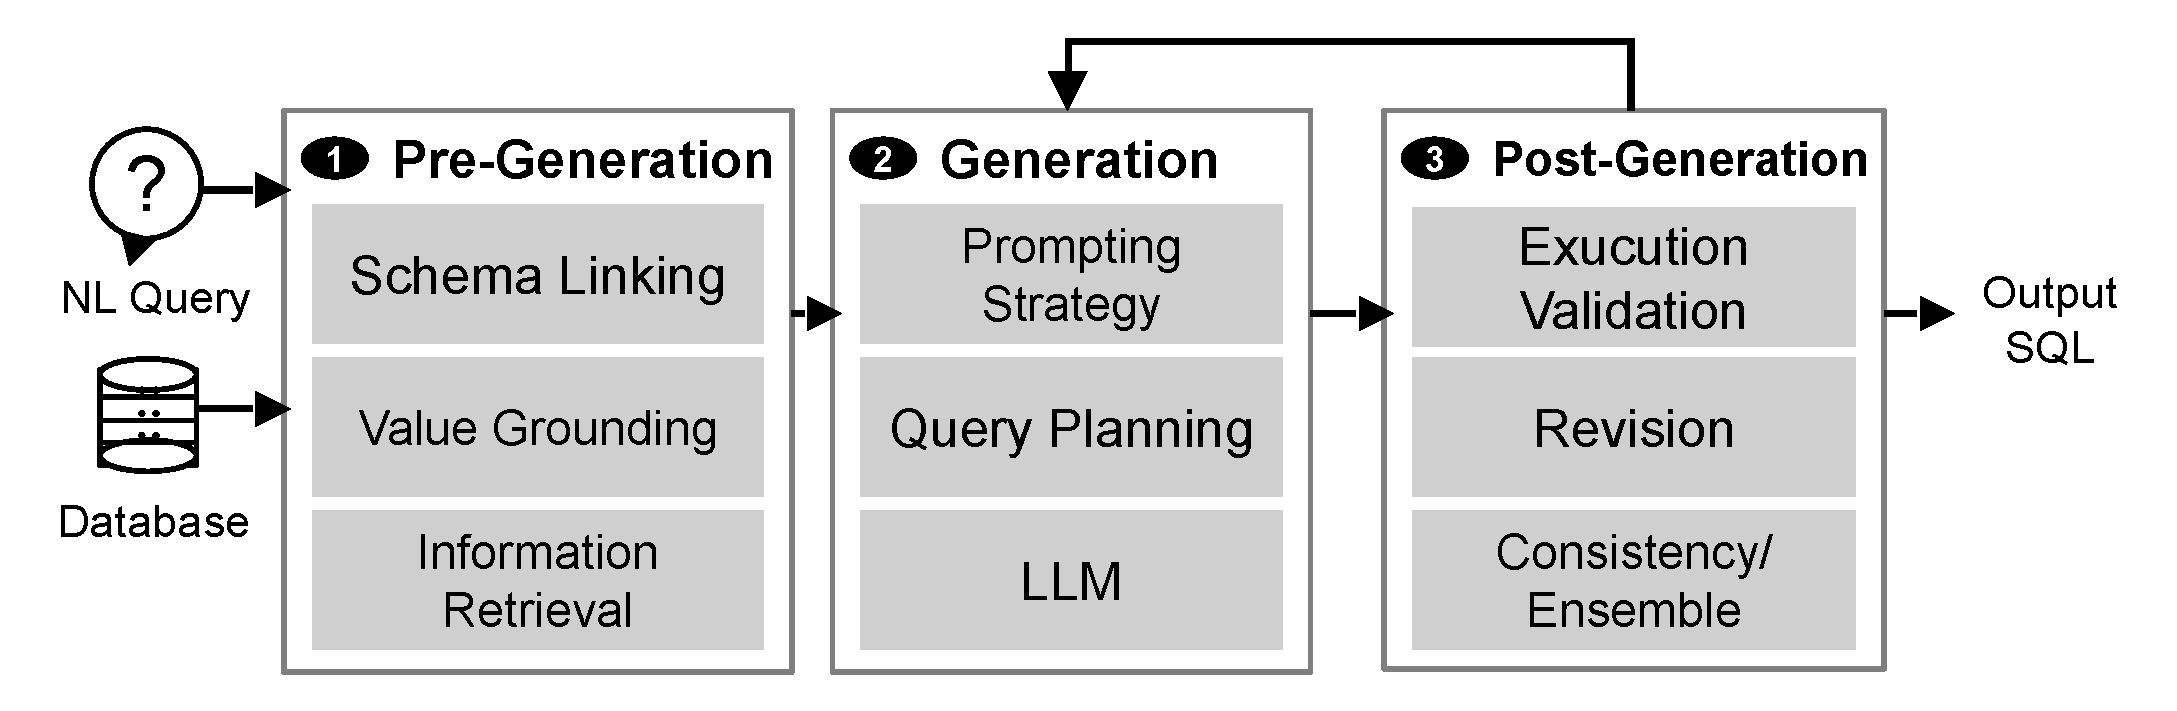
\includegraphics[width=1\linewidth]{./images/text-to-sql pipline.pdf} 
	\vspace{-5mm}
	\caption{\textbf{Overview of a typical Text-to-SQL pipeline, illustrating the Pre-Generation, Generation, and Post-Generation stages}}
	\label{fig:text-to-sql-pipeline}
	\vspace{-4mm}
\end{figure}

% 第3-5段，3个Limitations
%确实有一些工作开始做“自适应”，但多数只覆盖局部策略，而不是你这种结合环境感知、self-reflection、workflow/strategy selection 和 efficiency optimization 的 meta-cognitive controller。
%\textsc{CHESS} 会基于问题复杂度和上下文大小调整 schema pruning，但主要是 schema filtering 层面的自适应，不是全局 workflow selection。
%\textsc{QCMA-SQL} 明确做 question classification，并为不同复杂度问题调用不同 agents，比较接近“按难度选策略”。
%\textsc{OpenSearch-SQL} 提到 dynamic few-shot strategy 和 consistency alignment，更偏向 few-shot retrieval/selection 的局部自适应。
%还有一篇很新的 \textsc{SquRL} / “Beyond Static Pipelines” 直接批评 static pipeline，并通过强化学习学习动态 workflow；如果你后面 related work 要写，它可能需要重点区分。
%Although recent Text-to-SQL systems have introduced local adaptive mechanisms, such as difficulty-aware decomposition, adaptive schema pruning, dynamic demonstration retrieval, question-level agent routing, and even learned workflow policies, these adaptations are usually confined to specific stages of the pipeline.
%They provide limited support for jointly adapting the overall workflow, generation strategy, reflection behavior, and optimization effort according to the database environment, question difficulty, intermediate feedback, and execution efficiency.
% 我觉得需要讨论一下了
\textbf{L1: Limited Adaptation in Workflows and Strategy Selection.}
Many existing Text-to-SQL agents often predefine both the workflow structure and the strategy choices, where modules such as schema linking, few-shot retrieval, question decomposition, candidate generation, validation, and revision are applied in a largely fixed manner~\cite{gao2023text,pourreza2023din,wang2023mac,chaturvedi2025sqlthought,pham2026avsql}.
Although such designs improve robustness over single-shot generation, they provide limited support for adapting reasoning strategies to the current database environment, question difficulty, or intermediate feedback.
This can misallocate reasoning effort: simple queries over intuitive schemas may incur unnecessary token and latency overhead, while difficult queries may require deeper grounding, candidate comparison, or additional validation and reflection.
This mismatch is illustrated by the different effects of domain-specific hints in \textsc{BIRD}~\cite{li2023can}.
For an intuitive database such as \texttt{superhero}, where tables and columns are relatively descriptive, adding domain hints provides little additional benefit in our experiments.
In contrast, for a domain-heavy database such as \texttt{thrombosis\_prediction}, where terms such as \texttt{LDH} and gender-dependent uric-acid ranges require medical knowledge, the same hints improve accuracy from 20\% to nearly 50\%.
This contrast suggests that Text-to-SQL agents should adapt their grounding and generation strategies to the database environment, rather than applying the same strategy uniformly.

% 参考 MaCTG: Multi-Agent Collaborative Thought Graph for Automatic Programming
\textbf{L2: Post-hoc rather than Process-level Reflection.}
Feedback in many Text-to-SQL systems is mainly used after a candidate SQL has been generated, such as repairing execution errors, revising invalid queries, or selecting among completed candidates~\cite{pourreza2023din,wang2023mac,talaei2024chess,lei2024spider}.
Such feedback improves final-output validation, but provides limited support for monitoring and regulating the generation process itself.
In particular, the agent often lacks a controller that continuously tracks whether schema linking is reliable, whether candidate disagreement is increasing, whether repeated repairs are converging, or whether the current strategy should be changed.
As a result, early mistakes in schema linking, value grounding, or query planning may propagate into later steps and become cascading hallucinations.
Moreover, without global process supervision, local repair actions may fix surface-level execution errors while leaving the overall reasoning trajectory insufficiently grounded in the user question and database context.

\textbf{L3: Limited Awareness of Query Efficiency.}
Most existing Text-to-SQL systems are primarily optimized for correctness: they aim to generate SQL queries whose execution results match the ground-truth answers~\cite{li2023resdsql,li2024codes,li2023graphix,rai2023improving,scholak2021picard,wang2019rat,gao2023text,pourreza2023din}.
However, in practical database applications, a semantically correct SQL query is not necessarily efficient.
Equivalent or near-equivalent SQL formulations may lead to very different execution costs due to redundant projections, unnecessary joins, correlated subqueries, missing filter pushdown, suboptimal join orders, or functions applied to indexed columns~\cite{chaudhuri1998overview,leis2015good,wang2022wetune}.
Although database systems have long relied on rule-based, cost-based, and learned rewriting to improve query efficiency~\cite{selinger1979access,wang2022wetune,zhou2023learned,li2024llm}, current Text-to-SQL agents usually use database feedback mainly to check executability or result consistency.
They rarely treat execution plans, estimated costs, or bottleneck patterns as signals for deciding whether and how to rewrite the generated SQL.
As a result, the final query may be correct but unnecessarily expensive, especially in enterprise settings with large schemas, large tables, and long multi-step analytical workflows~\cite{lei2024spider}.


% 第六段  key insights
\textbf{Key Insights: Meta-cognitive and Environment-aware Text-to-SQL.}
Inspired by enactive cognition and meta-cognition, we view Text-to-SQL not as a static translation from question and schema to SQL, but as an adaptive interaction process between the agent and the database environment~\cite{varela1991embodied,flavell1979metacognition}.
Enactive cognition suggests that understanding is shaped through interaction with the environment, while meta-cognition emphasizes the ability to monitor and regulate one's own reasoning process.
In the context of Text-to-SQL, this means that an agent should perceive database-specific signals, act by generating and rewriting SQL, observe feedback from execution and query plans, and adjust its strategy when uncertainty, failure, or inefficiency is detected.
These perspectives lead to three design objectives.
First, to address \textbf{L1}, the agent should perform \emph{environment-aware workflow adaptation via strategy selection}: it should select lightweight or deep workflows according to the perceived database environment, question complexity, and intermediate feedback, rather than applying the same strategy uniformly.
Second, to address \textbf{L2}, the agent should support \emph{process-level self-reflection and dynamic control}: it should monitor schema-linking reliability, candidate disagreement, repair convergence, and strategy suitability during generation, so that early mistakes can be corrected before they propagate.
Third, to address \textbf{L3}, the agent should enable \emph{execution- and plan-aware SQL optimization}: it should use query plans, cost signals, semantic validation, and reusable rewrite knowledge to improve query efficiency while preserving correctness.

% 第七段 approach

% 第八段 evaluation

% 第九段 contributions

